\begin{document}
\chapter{Procesarea de imagini pe dispozitive mobile}
	Dispozitivele mobile au avut o evolutie constanta pe parcursul timpului. In ziua de astazi multe dintre aceste dispozitive mobile ating perfomante mult mai ridicate decat ale unor laptopuri cu o vechime de 10 ani. 
	Desi dispozitivele mobile sunt perfecte pentru realizarea unor activitati de zi cu zi si sunt capabile sa faca fata unor aplicatii costisitoare din punctul de vedere al complexitatii, forta lor de computatie este relativa slaba, in comparatie cu cea a calculatoarelor si a laptopurilor. Dispozitivele mobile nu profita de aceeasi cantitatea de memorie CPU si GPU de care profita calculatoarele si laptopurile, rezultand intr-o peroada de timp prelungita necesara pentru finalizarea antrenarii unui model de retele neuronale cu un numar mare de filtre, straturi si operatii, cum ar fi augmentarea datelor.
	
	\section{Istoria dispozitvelor mobile}
	Ideea telefoanelor fara fir a aparut inca din perioada primului razboi mondial, cand armata germana testa comunicarea independenta de fir in interioriul trenurilor militare. Dezvoltarea acestor dispozitive de comunicare a luat amploare foarte repede. In jurul anului 1940, in perioada celui de al doilea razboi mondial, emitatoarele radio portabile jucau un rol crucial in comunicarea armatei.
	Tehnologia de comunicare prin emitatoare radio folosita de armata, a inspirat mai departe compania de cercetare stiintifca Bell Labs in crearea dispozitivelor dependente de masina, in anul 1946. Prin intermediul acestor dispozitive devenea posibila comunicarea telefonica din interiorul masinilor (vezi Fig. \ref{fig:tanti-telefon}).
	
	\begin{figure}[H]
		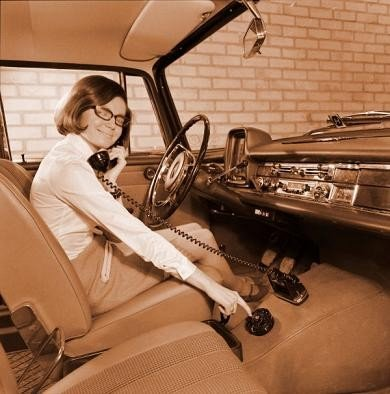
\includegraphics[width=10cm]{tanti-telefon}  
		\caption{\label{fig:tanti-telefon} Telefonul de masina creat de Bell Labs
			\protect
			\footnotemark}
	\end{figure}
	
	\footnotetext{http://www.realclear.com/offbeat/2016/02/03/\char`_did\char`_you\char`_know\char`_the\char`_first\char`_cell\char`_phone\char`_\\
		call\char`_was\char`_made\char`_out\char`_of\char`_spite\char`_12786.htm}
	
	La scurt timp dupa inovatia adusa de catre Bell Labs, AT\char`&T, compania americana specializata in telecomunicatii, va avea sa ofere servicii de telefonie mobila si canale de comunicare pe zone restranse. Dispozitivul oferit de catre AT\char`&T era asemanator un transmitator radio. Era necesara apasarea unui buton pentru a putea transmite un mesaj vocal, iar pentru a asculta interlocutorul, era necesara eliberarea butonului. Pentru a putea utiliza serviciile oferite de AT\char`&T in masina, era nevoie de atasarea unui echipament care cantarea aproximativ 36 de kg.
	In 1949, serviciul telefonic sustinut de AT\char`&T gazduia in jur de  5,000 de utilizatori, care realizau saptamanal aproximativ 30,000 de apeluri telefonice. Toate aceste apeluri telefonice erau gestionate manual de catre operatori ai companiei AT\char`&T. 
	
	Un serviciu asemanator celui oferit de AT\char`&T, a fost creat in Regatul Unit si se numea Post Office Radiophone Service. Diferenta facuta de acest serviciu telefonic a fost modul in care erau gestionate apeluri telefonice. Desi erau gestionate in continuare de un operator, un apel telefonic putea fi realizat intre oricare doi participanti din intregul Regat Unit. 
	
	Serviciul a fost creat in Manchester in 1959, adus in Londra in 1965, dupa care a fost distribuit in 1972 celorlalte orase mari din Anglia.
	In anul 1983 va avea sa apara primele telefoane mobile ce puteau fi tinute in mana. Primul producator de telefoane mobile a fost Motorola iar primul model a fost Motorola DynaTAC 8000x (vezi Fig.\ref{fig:dynatac}). Pretul sau crestea pana la 4000 de dolari, fiind un dispozitiv voluminos is greu (cantarind in jur de 4 kg)  avand o baterie capabila de a sustine 30 de minute de convorbire. In ciuda dimenisiunii mari a acestuia, era considerat cea mai buna varianta din punctul de vedere al portabilitatii datorita faptului ca va avea sa puna capat dependetei cablurilor telefonice pentru a purta o convorbire.
	
	\vfill
	
	\begin{figure}[H]
		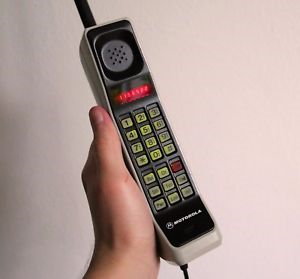
\includegraphics[width=8cm]{dynatac}  
		\caption{\label{fig:dynatac} Motorola DynaTAC 8000x
			\protect
			\footnotemark}
	\end{figure}
	
	\footnotetext{www.ebay.it}
	
	\vfill

	
	In anii 1990 au inceput sa aparata telefoane mobile apartinand generatiei a doua de dispozitive mobile. Acestea utilizau transmisie digitala, tehnologie ce aducea un plus de securitate si viteza peste transmisia analog. Odata cu aceasta generatie de dispozitive mobile, apar si SMS-urile (Short Message Service), prima utilizare fiind in 1993.
	In 1993, desi o teorie controversata, apare primul smartphone. IBM lanseaza modelul Simon. Acesta dispunea de: ceas, calendar, agenda telefonica, notite, casuta de email, auto-completare si touchscreen. (vezi Fig. \ref{fig:simon})
	
	
	
		\begin{figure}[H]
		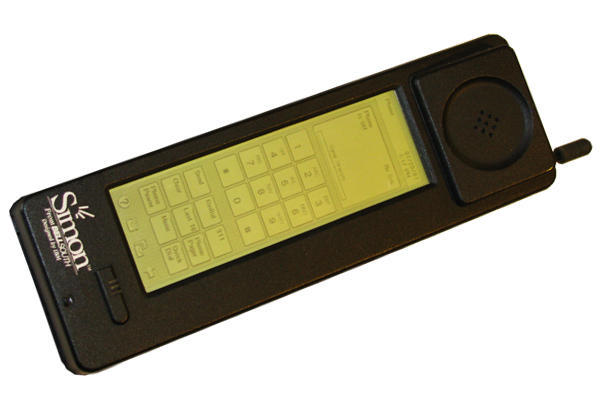
\includegraphics[width=8cm]{simon}  
		\caption{\label{fig:simon} Modelul de celular IBM Simon
			\protect
			\footnotemark}
	\end{figure}
	
	\footnotetext{shttps://www.androidauthority.com/ibm-simon-birthday-134255/}
	
	Dupa aparitia modelului Simon, creat de IBM, dispozitivele mobile vor avea sa urmeze un progres remarcabil in termen de functionalitate, stil si cel mai important, forta de computatie. 
	Telefoanele mobile au reusit sa introduca in buzunarul oamenilor forta de procesare, de la utilizarea unui simplu serviciu de email sau calendar, pana la utilizarea aplicatiilor ce dispun de inteligenta artificiala. \cite{history_cellphones}
	
	\vfill
	\section{Sistemul de operare Android}
	Android este un sistem de operare dezvoltat si intretinut de catre compania Google. Google a cumparat in anul 2005 compania Android Inc., o companie ce se ocupa cu sisteme de operare pentru camere foto digitale si telfoane mobile, cu scopul intrarii pe piata dispozitivelor mobile. Dupa 2 ani de la cumpararea companiei, Google lanseaza sistemul de operare pe piata. 
	
	In momentul de fata, 85\% din totalitatea utilizatorilor dispozitivelor mobile smartphone, utlizeaza sistemul de operare Android. 
	Ceea ce face sistemul de operare Android, un punct de interes in viziunea invatarii automate, este arhitectura sa. Android are la baza o versiune a nucleului Linux, sistem de operare care face parte din familia UNIX. Sistemul de operare poate rula pe arhitecturi ARM dar si x86 si x86-x64 in perioada ce va urma. 
	
	Incepand din anul 2012, dispozitivele mobile Android sunt dezvoltate utliziand procesoare Intel iar mai tarziu se vor stabili pe arhitecturi de 64-bit, ARM64. 
	Forta pe care procesoarele dispozitivelor mobile o aduc, impreuna cu sistemul de operare Android, ne permit utilizarea multor tehnici de invatare automata chiar pe sistemul telefonului. 
	
	

\end{document}